\begin{center}\section{定积分}\label{chapter_definite_integral}\end{center}
\subsection{定积分的定义}
\begin{minipage}{.5\textwidth}
	\begin{center}
		$\left[a,b\right]\mbox{有限区间,},f(x)\mbox{在}\left[a,b\right]\mbox{上有界}$\\
		$\left[a,b\right]\mbox{内任找}n-1\mbox{个点,}\mbox{分成$n$个区间}$\\
		$a=x_0<x_1<x_2\cdots x_{n-1}<x_{n}=b$\\
		$\left[x_0,x_1\right],\left[x_1,x_2\right]\cdots\left[x_{n-1},x_n\right]$\\
		$\mbox{分成$n$个曲边梯形,}\left[x_{i-1},x_i\right]\mbox{为第$i$个}$\\
		$\mbox{面积}\vartriangle S_i,\mbox{对应底}\vartriangle x_i=x_i-x_{i-1}$\\
		$\forall \xi_i \in \left[x_{i-1},x_i\right],\vartriangle S_i \approx f(\xi_i)\vartriangle x_i$\\
		$S=\vartriangle S_1+\vartriangle S_2\cdots\vartriangle S_n=\sum\limits_{i=1}^{n}f(\xi_i)\vartriangle x_i$\\
		$\lambda=\max\left\{\vartriangle x_1,\vartriangle x_2,\cdots,\vartriangle x_n\right\},\mbox{当}\lambda\rightarrow 0\mbox{时}$
	\end{center}
\end{minipage}
\hfill
\vline
\begin{minipage}{.5\textwidth}
\begin{center}
	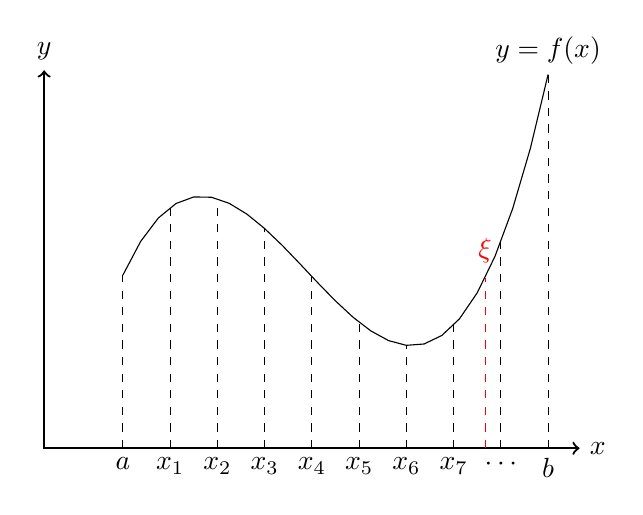
\begin{tikzpicture}[xscale=2,yscale=1.6]
		\draw[<->,thick](0,3)node[above]{$y$}--(0,0)--(3.4,0)node[right]{$x$};
		\draw[domain=-.5:2.2]plot(\x+1,{(\x)^3-2*(\x)^2+2});
		\draw[dashed] (.5,0)node[below]{$a$}--(.5,{(-.5)^3-2*(-.5)^2+2});
		\draw[dashed] (3.2,0)node[below]{$b$}--(3.2,{(2.2)^3-2*(2.2)^2+2})node[above]{$y=f(x)$};
		\foreach[count=\i] \x in {.8,1.1,...,2.7}
		\draw[dashed] (\x,0)node[below]{$x_\i$}--(\x,{(\x-1)^3-2*(\x-1)^2+2});
		\draw[dashed] (3.2-.3,0)node[below]{$\cdots$}--(3.2-.3,{(2.2-.3)^3-2*(2.2-.3)^2+2});
		\draw[dashed,color=red] (2.8,0)--(2.8,{(1.8)^3-2*(1.8)^2+2})node[above=2]{$\xi$};
	\end{tikzpicture}
\end{center}
\end{minipage}
	$$S=\lim\limits_{\lambda \to 0}\sum\limits_{i=1}^{n}f(\xi_i)\vartriangle x_i$$
	$$S\mbox{是一个定数,则称}f(x)\mbox{在}\left[a,b\right]\mbox{上可积,}S\mbox{称为}f(x)\mbox{在}\left[a,b\right]\mbox{上的定积分记作:}$$
	$$\int_{a}^{b}f(x)\ dx\begin{cases}
		f(x) \ dx &\mbox{被积表达式}\begin{cases}
			f(x) &\mbox{被积函数}
		\end{cases}\\
		x &\mbox{积分变量}\\
		\left[a,b\right]&\mbox{积分区间}\begin{cases}
				a &\mbox{积分下限}\\  
			b &\mbox{积分上限}
		\end{cases}
	\end{cases}$$
	$$\ \int_{a}^{b}f(x) \ dx\triangleq\lim\limits_{\lambda \to 0}\sum_{i=1}^{n}f(\xi_i)\vartriangle x_i$$
\subsection{可积的充分条件}
	\begin{align}
			&\mbox{如果}f(x)\mbox{在}\left[a,b\right]\mbox{上连续,则}f(x)\mbox{在}\left[a,b\right]\mbox{上可积}\\
			&\mbox{如果}f(x)\mbox{在}\left[a,b\right]\mbox{上有界,且至多有有限个间断点,则}f(x)\mbox{在}\left[a,b\right]\mbox{上可积}
	\end{align}
\subsection{定积分的性质}
	\centerline{$a<b<c,k\mbox{为常数}$}
	\begin{align}	
		\int_{a}^{a}f(x)\ dx&=0 \label{Definite_integral_property_1}\\
		\int_{a}^{b}\ dx &=b-a \label{Definite_integral_property_2}\\
		\int_{a}^{b}f(x)\ dx&=-\int_{b}^{a}f(x)\ dx \label{Definite_integral_property_3}\\
		\int_{a}^{c}f(x)\ dx&=\int_{a}^{b} f(x)\ dx+\int_{b}^{c}f(x)\ dx \label{Definite_integral_property_4}\\
		\int_{a}^{b}f(x)\ dx&=\int_{a}^{c}f(x)\ dx+\int_{c}^{b}f(x)\ dx \label{Definite_integral_property_5}\\
		\int_{a}^{b}kf(x)\ dx&=k\int_{a}^{b}f(x)\ dx \label{Definite_integral_property_6}\\
		\int_{a}^{b}f(x)\pm g(x)\ dx&=\int_{a}^{b}f(x)\ dx\pm \int_{a}^{b}g(x)\ dx\label{Definite_integral_property_7} \\
		f(x)\geqslant 0\quad &\Rightarrow \int_{a}^{b}f(x)\ dx\geqslant 0 \label{Definite_integral_property_8}\\
		f(x)\geqslant g(x)\quad &\Rightarrow \int_{a}^{b}f(x)\ dx\geqslant \int_{a}^{b}g(x)\ dx \label{Definite_integral_property_9}\\
		\left|\int_{a}^{b}f(x) \ dx\right|&\leqslant \int_{a}^{b}\left|f(x)\right|\ dx \label{Definite_integral_property_10}
	\end{align}
\subsection{积分估值公式}
	$$M\mbox{为区间$\left[a,b\right]$最大值},m\mbox{为区间$\left[a,b\right]$最小值},a<b$$
	\begin{equation}
		m(b-a)\leqslant \int_{a}^{b}f(x)\ dx\leqslant M(b-a)\label{Integral_valuation_formula}
	\end{equation}
\subsection{积分中值定理}
	$$f(x)\mbox{是}\left[a,b\right]\mbox{上的连续函数,则},\exists \xi \in\left[a,b\right],a<b\mbox{使}$$
	\begin{equation}
		\int_{a}^{b}f(x)\ dx= f(\xi)(b-a) \label{Integral_mean_value_theorem}
	\end{equation}
	$$f(\xi)=\frac{1}{b-a}\int_{a}^{b}f(x)\ dx\qquad\mbox{称为均值}$$
\subsection{积分上限函数}
\subsubsection{定义}
\begin{minipage}{.5\textwidth}
	\begin{center}
		$x\in \left[a,b\right],\left[a,x\right]\mbox{对应曲边梯形}$\\
		$\int_{a}^{x}f(x)\ dx=\int_{a}^{x}f(u)\ du$\\
		$\phi(x)\triangleq\int_{a}^{x}f(u)\ du$\\
		$\phi(x)\mbox{是}\left[a,b\right]\mbox{上函数称为积分上限函数}$
	\end{center}
\end{minipage}
\hfill
\vline
\begin{minipage}{.5\textwidth}
	\begin{center}
		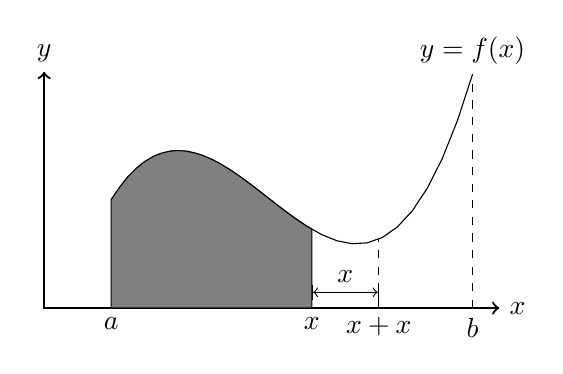
\begin{tikzpicture}[xscale=1.7]
			\draw[thick,<->,thick](0,3)node[above]{$y$}--(0,0)--(3.4,0)node[right]{$x$};
			\draw[domain=-.5:2.2]plot(\x+1,{(\x)^3-2*(\x)^2+2});
			\draw[dashed] (.5,0)coordinate (a)node[below]{$a$}--(.5,{(-.5)^3-2*(-.5)^2+2});
			\draw[dashed] (2.5,0)node[below]{$x+\vartriangle x$}--(2.5,{(1.5)^3-2*(1.5)^2+2});
			\draw[|<->|] (2,.2)--node[above]{$\vartriangle x$}(2.5,.2);
			\draw[dashed] (3.2,0)node[below]{$b$}--(3.2,{(2.2)^3-2*(2.2)^2+2})node[above]{$y=f(x)$};
			\draw[dashed] (2,0)coordinate (x)node[below]{$x$}--(2,{(1)^3-2*(1)^2+2});
			\draw[domain=-.5:1,fill=gray](a)--plot(\x+1,{(\x)^3-2*(\x)^2+2})--(x)--(a);
		\end{tikzpicture}
	\end{center}
\end{minipage}
\subsubsection{性质}
	\begin{align}
		\phi'(x)=\frac{d}{dx}\left[\int_{a}^{x}f(u)\ du\right]&=f(x)\label{integral_upper_limit_function_1}\\
		\frac{d}{dx}\left[\int_{a}^{\psi(x)}f(u)\ du\right]&=f(\psi(x))\psi'(x)\label{integral_upper_limit_function_2}\\
		\frac{d}{dx}\left[\int_{v(x)}^{\psi(x)}f(u)\ du\right]&=f\left[\psi(x)\right]\psi'(x)-f\left[v(x)\right]v'(x)\label{integral_upper_limit_function_3}
	\end{align}
	\begin{center}
			若$f(x)$在$\left[a,b\right]$上连续,则$f(x)$必存在原函数,$\phi(x)=\int_{a}^{x}f(u)\ du$\\
			即为$f(x)$在$\left[a,b\right]$上的一个原函数
			$$\int f(x)\ dx=\int_{a}^{x}f(u)\ du+C$$
	\end{center}
\subsection{微积分基本公式(牛顿莱布兹尼公式)}
	\centerline{$f(x)$在$\left[a,b\right]$上连续,F(x)是f(x)在$\left[a,b\right]$上的的一个原函数}
	\begin{equation}
		\int_{a}^{b}f(x)\ dx=F(b)-F(a) \triangleq \left[F(x)\right]_a^b=\left.F(x)\right|_a^b\label{Leibniz_formula}
	\end{equation}
\subsection{换元法}
	\begin{center}
		$f(x)$在$\left[a,b\right]$上连续,$x=\varphi(t)\begin{cases}
			\varphi(\alpha)=a\\
			\varphi(\beta)=b
		\end{cases}$\\
	$\varphi(t)\mbox{在}\left[\alpha,\beta\right]\mbox{上有连续导数,且}R_\varphi=\left[a,b\right]$
	\end{center}
	\begin{equation}
		\int_{a}^{b}f(x)\ dx=\int_{\alpha}^{\beta}f\left[\varphi(t)\right]\varphi'(t)\ dt\label{Fixed_integral_substitution_method}
	\end{equation}
\subsection{分部积分法}
\begin{equation}
	\int_{a}^{b}u\ dv=\left[uv\right]_a^b-\int_{a}^{b}v\ du
\end{equation}
\subsection{奇偶函数积分}
	\begin{align}
	(\mbox{奇函数})\quad	&\int_{-a}^{a}f(x)\ dx=2\int_{0}^{a}f(x)\ dx\label{Odd_even_function_integral_1}\\
	(\mbox{偶函数})\quad	&\int_{-a}^{a}f(x)\ dx=0\label{Odd_even_function_integral_2}
	\end{align}
\subsection{周期函数积分}
	\begin{align}
		\int_{a}^{a+T}f(x)\ dx&=\int_{0}^{T}f(x)\ dx\label{Periodic_function_integral_1}\\
		\int_{a}^{a+nT}f(x)\ dx&=n\int_{0}^{T}f(x)\ dx\label{Periodic_function_integral_2}
	\end{align}
\subsection{积分定理}
\begin{align}
	\int_{0}^{\frac{\pi}{2}}f(\sin x)\ dx&=\int_{0}^{\frac{\pi}{2}}f(\cos x)\ dx\label{Definite_integral_theorem_1}\\
	\int_{0}^{\frac{\pi}{2}}\sin^n x\ dx=\int_{0}^{\frac{\pi}{2}}\cos^n x\ dx&=\begin{cases}
				\frac{n-1}{n}\cdot\frac{n-3}{n-2}\cdots\frac{3}{4}\cdot\frac{1}{2}\cdot\frac{\pi}{2}\quad(\mbox{n偶数})\\
		\frac{n-1}{n}\cdot\frac{n-3}{n-2}\cdots\frac{4}{5}\cdot\frac{2}{3}\cdot 1\quad(\mbox{n奇数})
	\end{cases}\label{Definite_integral_theorem_2}
\end{align}
\subsection{积分不等式}
\begin{align}
	\left[\int_{a}^{b}f(x)g(x)\ dx\right]^2&\leqslant \int_{a}^{b}f^2(x)\ dx\cdot \int_{a}^{b}g^2(x)\ dx \label{Definite_integral_inequality_1}\\
	\left\{\int_{a}^{b}\left[f(x)+g(x)\right]^2 \ dx\right\}^{\frac{1}{2}}&\leqslant \left[\int_{a}^{b}f^2(x)\ dx\right]^{\frac{1}{2}}+\left[\int_{a}^{b}g^2(x)\ dx\right]^{\frac{1}{2}}\label{Definite_integral_inequality_2}
\end{align}
\subsection{一些废话(显而易见的东西)}
	\begin{align}
		\mbox{若在}\left[a,b\right]\mbox{上}f(x)\geqslant 0,\mbox{且}\int_{a}^{b}f(x)\ dx = 0,\mbox{则}f(x)\equiv 0 \label{Definite_integral_identity_1}\\
		\mbox{若在}\left[a,b\right]\mbox{上}f(x)\geqslant 0,\mbox{且}f(x)\not\equiv 0,\mbox{则}\int_{a}^{b}f(x)\ dx > 0 \label{Definite_integral_identity_2}
	\end{align}
	\begin{equation}
			\mbox{若在}\left[a,b\right]\mbox{上}f(x)\leqslant g(x),\mbox{且}\int_{a}^{b}f(x)\ dx=\int_{a}^{b}g(x)\ dx\mbox{则}f(x)=g(x),x\in\left[a,b\right] \label{Definite_integral_identity_3}
	\end{equation}
